\documentclass[11pt]{beamer}
% Classic university style: Madrid theme, 4:3.
% Speaker notes: \note{} on each content slide. To show them, add
%   \setbeameroption{show notes on second screen=right}
\usetheme{Madrid}
\setbeamertemplate{navigation symbols}{}
\setbeamertemplate{theorems}[numbered]

\usepackage{amsmath,amssymb}
\usepackage{booktabs}
\usepackage{siunitx}
\sisetup{exponent-product=\times}

% Auto-generated by scripts/export_macros.py from results/results.json. Do not edit.
\newcommand{\Kval}{\num{100}}
\newcommand{\rval}{\num{0.05}}
\newcommand{\sigmaval}{\num{0.25}}
\newcommand{\Tval}{\num{1}}
\newcommand{\Bone}{\num{80}}
\newcommand{\Btwo}{\num{130}}
\newcommand{\kval}{\num{1.6}}
\newcommand{\alphaval}{\num{-0.3}}
\newcommand{\betaval}{\num{-1.69}}
\newcommand{\taufinal}{\num{0.03125}}
\newcommand{\priceEighty}{\num{3.1415}}
\newcommand{\priceNinety}{\num{6.8698}}
\newcommand{\priceHundred}{\num{12.3360}}
\newcommand{\priceHundredTen}{\num{19.3051}}
\newcommand{\priceHundredTwenty}{\num{27.4063}}
\newcommand{\TableMethodsRows}{80 & \num{3.1415} & \num{3.1415} & \num{3.1398} & \num{3.1403} & \num{3.150} & [\num{3.133}, \num{3.168}] \\
90 & \num{6.8698} & \num{6.8698} & \num{6.8686} & \num{6.8675} & \num{6.888} & [\num{6.861}, \num{6.914}] \\
100 & \num{12.3360} & \num{12.3360} & \num{12.3351} & \num{12.3332} & \num{12.360} & [\num{12.324}, \num{12.396}] \\
110 & \num{19.3051} & \num{19.3051} & \num{19.3043} & \num{19.3026} & \num{19.335} & [\num{19.290}, \num{19.380}] \\
120 & \num{27.4063} & \num{27.4063} & \num{27.4054} & \num{27.4046} & \num{27.441} & [\num{27.387}, \num{27.494}] \\}
\newcommand{\errHeatKernel}{\num{2.5e-14}}
\newcommand{\errExplicit}{\num{0.0017}}
\newcommand{\errCN}{\num{0.0028}}
\newcommand{\errMC}{\num{0.034}}
\newcommand{\mcCoverCount}{5}
\newcommand{\mcSeMax}{\num{0.027}}
\newcommand{\fdDx}{\num{0.0125}}
\newcommand{\fdLam}{\num{0.4}}
\newcommand{\cnSteps}{\num{400}}
\newcommand{\mcPaths}{\num{1e6}}
\newcommand{\parityGap}{\num{5.7e-14}}
\newcommand{\stabDx}{\num{0.0125}}
\newcommand{\stabErrThirty}{\num{0.0016}}
\newcommand{\stabErrForty}{\num{0.0018}}
\newcommand{\stabErrHalf}{\num{0.0066}}
\newcommand{\stabErrFiftyTwo}{\num{2.2e10}}
\newcommand{\stabErrFiftyFive}{\num{2.2e26}}
\newcommand{\stabErrSixty}{\num{5.7e46}}
\newcommand{\TableStabilityRows}{0.3 & \num{0.2999} & 667 & \num{1} & \num{0.0016} \\
0.4 & \num{0.4000} & 500 & \num{1} & \num{0.0018} \\
0.5 & \num{0.5000} & 400 & \num{1} & \num{0.0066} \\
0.52 & \num{0.5195} & 385 & \num{1.08} & \num{2.2e10} \\
0.55 & \num{0.5495} & 364 & \num{1.2} & \num{2.2e26} \\
0.6 & \num{0.6006} & 333 & \num{1.4} & \num{5.7e46} \\}
\newcommand{\convOrderMax}{2.00}
\newcommand{\convOrderK}{2.00}
\newcommand{\convLocalMin}{2.000}
\newcommand{\convLocalMax}{2.002}
\newcommand{\TableConvergenceRows}{\num{0.025} & 125 & \num{0.00741} & \num{0.0035} \\
\num{0.0125} & 500 & \num{0.00185} & \num{8.79e-4} \\
\num{0.00625} & 2000 & \num{4.62e-4} & \num{2.20e-4} \\
\num{0.003125} & 8000 & \num{1.16e-4} & \num{5.50e-5} \\
\num{0.0015625} & 32000 & \num{2.89e-5} & \num{1.38e-5} \\}
\newcommand{\convErrFinest}{\num{2.9e-5}}
\newcommand{\convOrderOff}{2.00}
\newcommand{\convLocalOffMin}{2.00}
\newcommand{\convLocalOffMax}{2.00}
\newcommand{\convErrOffFinest}{\num{2.7e-5}}
\newcommand{\barA}{\num{-0.2231}}
\newcommand{\barB}{\num{0.2624}}
\newcommand{\barEll}{\num{0.4855}}
\newcommand{\barDiffMax}{\num{1.1e-5}}
\newcommand{\TableBarrierRows}{85 & \num{0.7610} & \num{4.7841} \\
90 & \num{1.3657} & \num{6.8698} \\
100 & \num{1.9621} & \num{12.3360} \\
110 & \num{1.7492} & \num{19.3051} \\
120 & \num{0.9755} & \num{27.4063} \\
125 & \num{0.4911} & \num{31.7656} \\}
\newcommand{\barPriceHundred}{\num{1.9621}}
\newcommand{\termsShortest}{51}
\newcommand{\termsLongest}{2}
\newcommand{\termsShortestDays}{1}
\newcommand{\termsPredShortest}{51}
\newcommand{\termsPredLongest}{2.7}
\newcommand{\nnPlainRmseTwenty}{\num{0.78}}
\newcommand{\nnPinnRmseTwenty}{\num{0.021}}
\newcommand{\nnPlainResTwenty}{\num{0.033}}
\newcommand{\nnPinnResTwenty}{\num{6.6e-4}}
\newcommand{\nnRmseRatioTwenty}{37}
\newcommand{\nnResRatioTwenty}{50}
\newcommand{\nnPinnSecondsTwenty}{111}
\newcommand{\nnPlainRmseFifty}{\num{0.31}}
\newcommand{\nnPinnRmseFifty}{\num{0.028}}
\newcommand{\nnPlainResFifty}{\num{0.017}}
\newcommand{\nnPinnResFifty}{\num{7.4e-4}}
\newcommand{\nnRmseRatioFifty}{11}
\newcommand{\nnResRatioFifty}{22}
\newcommand{\nnPinnSecondsFifty}{102}
\newcommand{\nnPlainRmseTwoHundred}{\num{0.2}}
\newcommand{\nnPinnRmseTwoHundred}{\num{0.026}}
\newcommand{\nnPlainResTwoHundred}{\num{0.014}}
\newcommand{\nnPinnResTwoHundred}{\num{7.7e-4}}
\newcommand{\nnRmseRatioTwoHundred}{8}
\newcommand{\nnResRatioTwoHundred}{18}
\newcommand{\nnPinnSecondsTwoHundred}{119}
\newcommand{\TableNNRows}{20 & \num{0.78} $\pm$ \num{0.2} & \num{0.021} $\pm$ \num{0.01} & \num{0.033} & \num{6.6e-4} \\
50 & \num{0.31} $\pm$ \num{0.1} & \num{0.028} $\pm$ \num{0.01} & \num{0.017} & \num{7.4e-4} \\
200 & \num{0.2} $\pm$ \num{0.07} & \num{0.026} $\pm$ \num{0.01} & \num{0.014} & \num{7.7e-4} \\}
\newcommand{\TableNNRowsShort}{20 & \num{0.78} & \num{0.021} & \num{0.033} & \num{6.6e-4} \\
50 & \num{0.31} & \num{0.028} & \num{0.017} & \num{7.4e-4} \\
200 & \num{0.2} & \num{0.026} & \num{0.014} & \num{7.7e-4} \\}
\newcommand{\nnAdamIters}{\num{10000}}
\newcommand{\nnLbfgsIters}{\num{3000}}
\newcommand{\nnColloc}{\num{4096}}
\newcommand{\nnTerminal}{\num{400}}
\newcommand{\nnBoundary}{\num{200}}
\newcommand{\nnSeeds}{3}
\newcommand{\nnWidth}{32}
\newcommand{\nnDepth}{3}
\newcommand{\nnLr}{\num{0.002}}
\newcommand{\nnSmax}{\num{2}}
\newcommand{\nnThetaMin}{\num{0.02}}
\newcommand{\nnTestGrid}{60}
\newcommand{\illEps}{\num{1.00e-6}}
\newcommand{\illModes}{127}
\newcommand{\illMaxNoisyHalfMilli}{\num{1}}
\newcommand{\illMaxNoisyOneMilli}{\num{2.8}}
\newcommand{\illMaxNoisyTwoMilli}{\num{1.3e7}}
\newcommand{\illAmpOneMilli}{\num{1.0e7}}
\newcommand{\illMaxCleanThreeMilli}{\num{1.2e+03}}
\newcommand{\hadTwentyData}{\num{0.05}}
\newcommand{\hadTwentySol}{\num{1.2e16}}

\newcommand{\N}{\mathcal N}
\newcommand{\dd}{\,\mathrm d}
\graphicspath{{../figures/}}

\title[Black--Scholes = Heat Equation]{Black--Scholes is the Heat Equation in Disguise}
\subtitle{MA5030 Partial Differential Equations}
\author[Goyal \& Bindal]{Harshil Goyal (ES23BTECH11016)\\Amogh Bindal (ES23BTECH11004)}
\institute[IIT Hyderabad]{Indian Institute of Technology Hyderabad}
\date{\today}

\begin{document}

% =====================================================================
\begin{frame}
  \titlepage
\end{frame}

\begin{frame}{Outline}
  \tableofcontents
  \note{We first build the Black--Scholes equation from scratch, then classify it and transform it step by
  step into the heat equation. We solve the heat equation with full proofs and recover the Black--Scholes
  formula. Finally we use the same idea for barrier options, numerics and neural networks.}
\end{frame}

% =====================================================================
\section{The Black--Scholes equation}

\begin{frame}{What is a European call option?}
  \begin{columns}[c]
    \begin{column}{0.48\textwidth}
      \begin{itemize}
        \item Right (not obligation) to \textbf{buy} one share at strike $K$ on expiry date $T$.
        \item Value at expiry:
        \[ V(S,T)=\max(S-K,0) \]
        \item Question: what is it worth at $t<T$?
      \end{itemize}
      \vspace{4pt}
      {\small $K=\Kval$, $r=\rval$, $\sigma=\sigmaval$, $T=\Tval$.}
    \end{column}
    \begin{column}{0.52\textwidth}
      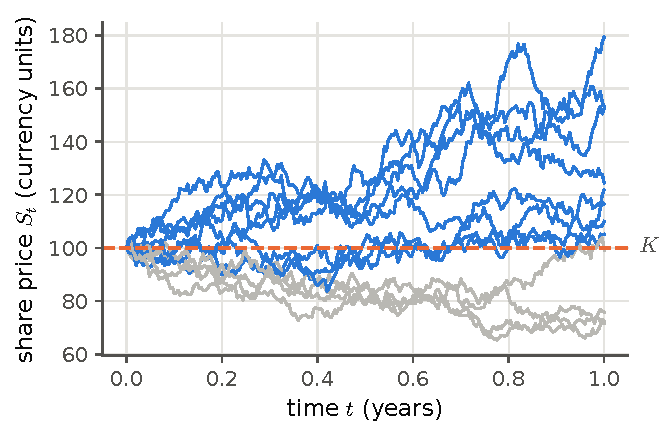
\includegraphics[width=\textwidth]{fig_paths.pdf}\\
      {\scriptsize Simulated share prices; blue paths end above $K$ and pay off.}
    \end{column}
  \end{columns}
  \note{A call is the right to buy at the strike price at expiry, so at expiry it is worth max(S-K,0).
  Before expiry the future share price is random, as the simulated paths show, so we need a model of the
  share price to price the option today. These are the default parameters for every number in the talk.}
\end{frame}

\begin{frame}{Model for the share price}
  \textbf{Geometric Brownian motion:}
  \[
    \dd S=\mu S\dd t+\sigma S\dd W
  \]
  \begin{itemize}
    \item $\mu$: drift, \ $\sigma$: volatility, \ $W$: Brownian motion, \ $(\dd W)^2=\dd t$.
    \item Bank account grows at constant rate $r$.
  \end{itemize}
  \vspace{4pt}
  \textbf{Itô's lemma} (taken as given): for smooth $V(S,t)$,
  \[
    \dd V=V_t\dd t+V_S\dd S+\tfrac12V_{SS}(\dd S)^2,\qquad (\dd S)^2=\sigma^2S^2\dd t,
  \]
  \[
    \Rightarrow\quad \dd V=\Big(V_t+\mu SV_S+\tfrac12\sigma^2S^2V_{SS}\Big)\dd t+\sigma SV_S\dd W .
  \]
  \note{The share price grows at rate mu on average with random fluctuations proportional to its level.
  Itô's lemma is the chain rule for random processes: because dW squared equals dt, the second derivative
  term survives at first order in dt.}
\end{frame}

\begin{frame}{Derivation: delta hedging}
  Portfolio: one option, short $\Delta$ shares, \ $\Pi=V-\Delta S$.
  {\small
  \[
    \dd\Pi=\dd V-\Delta\dd S
    =\Big(V_t+\mu SV_S+\tfrac12\sigma^2S^2V_{SS}-\mu\Delta S\Big)\dd t+\sigma S(V_S-\Delta)\dd W
  \]}
  \begin{enumerate}
    \item Choose $\Delta=V_S$: random term vanishes, and so does $\mu$.
    \item Riskless $\Rightarrow$ earns bank rate (no arbitrage): $\dd\Pi=r\Pi\dd t=r(V-SV_S)\dd t$.
    \item Equate the two expressions for $\dd\Pi$:
  \end{enumerate}
  \begin{block}{Black--Scholes equation}
    \[
      V_t+\tfrac12\sigma^2S^2V_{SS}+rSV_S-rV=0,\qquad S>0,\ t<T
    \]
  \end{block}
  \note{We hold one option and sell V_S shares. The random terms cancel exactly, and with them the unknown
  drift mu, which is why the price does not depend on investors' expectations. A riskless portfolio must
  earn the bank rate, and equating the two expressions gives the Black--Scholes equation.}
\end{frame}

\begin{frame}{The complete problem}
  \[
    \underbrace{V_t}_{\text{time decay}}
    +\underbrace{\tfrac12\sigma^2S^2V_{SS}}_{\text{diffusion}}
    +\underbrace{rSV_S}_{\text{drift}}
    -\underbrace{rV}_{\text{discounting}}=0
  \]
  \vspace{4pt}
  \begin{center}
  \begin{tabular}{ll}
    Terminal condition: & $V(S,T)=\max(S-K,0)$\\[4pt]
    Boundary at $S=0$: & $V(0,t)=0$\\[4pt]
    Boundary as $S\to\infty$: & $V(S,t)\sim S-Ke^{-r(T-t)}$
  \end{tabular}
  \end{center}
  \vspace{6pt}
  \begin{itemize}
    \item Data given at the \emph{final} time $T$; solve backwards to today.
    \item Variable coefficients $S^2$, $S$: not yet a textbook equation.
  \end{itemize}
  \note{Each term has a meaning: diffusion from the randomness, drift from interest, and discounting. The
  data are given at expiry and we need the value today, so we solve backwards in time. The coefficients
  depend on S, which is what the change of variables will remove.}
\end{frame}

% =====================================================================
\section{Classification and reduction to the heat equation}

\begin{frame}{Classification of second-order PDEs}
  General linear equation in two variables $(X,Y)$:
  \[
    A\,w_{XX}+2B\,w_{XY}+C\,w_{YY}+(\text{lower order})=0
  \]
  \begin{center}
  \begin{tabular}{lll}
    \toprule
    $B^2-AC>0$ & hyperbolic & wave equation\\
    $B^2-AC=0$ & parabolic & heat equation\\
    $B^2-AC<0$ & elliptic & Laplace equation\\
    \bottomrule
  \end{tabular}
  \end{center}
  \begin{itemize}
    \item The type is invariant under smooth invertible changes of variables.
    \item Characteristics: $A\dd Y^2-2B\dd X\dd Y+C\dd X^2=0$.
    \item Parabolic canonical form: $w_{\xi\xi}+(\text{lower order})=0$.
  \end{itemize}
  \note{This is the classification from Myint-U and McOwen. The sign of the discriminant decides the type,
  and the type does not change under a change of variables. For parabolic equations only one second
  derivative survives in canonical form.}
\end{frame}

\begin{frame}{Black--Scholes is parabolic}
  With $(X,Y)=(S,t)$, the principal part is $\tfrac12\sigma^2S^2V_{SS}$:
  \[
    A=\tfrac12\sigma^2S^2,\quad B=0,\quad C=0\quad\Rightarrow\quad B^2-AC=0 .
  \]
  \begin{itemize}
    \item \textbf{Parabolic} for every $S>0$; characteristics $A\dd t^2=0$: lines $t=$ const.
    \item \textbf{Degenerate} at $S=0$: $A=B=C=0$, the PDE becomes $V_t=rV$, which forces $V(0,t)=0$.
    \item \textbf{Backward}: $V_t$ and $V_{SS}$ have the same sign, so it is well posed for decreasing $t$.
  \end{itemize}
  \vspace{4pt}
  Forward in $t$ it is the backward heat equation (ill posed):
  \[
    w_t=-w_{xx},\ \ w(x,0)=\tfrac1n\sin nx\ \Rightarrow\ w=\tfrac1n e^{+n^2t}\sin nx\to\infty .
  \]
  \note{Only V_SS appears, so the discriminant is zero. At S equals zero the principal part vanishes and the
  equation reduces to an ODE, which supplies the boundary condition. Solving in the wrong direction is
  Hadamard ill posed: arbitrarily small data give arbitrarily large solutions.}
\end{frame}

\begin{frame}{Step 1: logarithmic price, $S=Ke^x$}
  Let $x=\ln(S/K)$ and $V(S,t)=K\,v(x,\tau)$. Since $\frac{\dd x}{\dd S}=\frac1S$:
  \[
    V_S=\frac{K}{S}v_x\quad\Rightarrow\quad SV_S=K\,v_x .
  \]
  Differentiate $SV_S=Kv_x$ once more with respect to $S$:
  \[
    V_S+SV_{SS}=\frac{K}{S}v_{xx}\quad\Rightarrow\quad S^2V_{SS}=K\,(v_{xx}-v_x).
  \]
  \begin{alertblock}{Effect}
    $S\partial_S\to\partial_x$: the variable coefficients $S^2$ and $S$ disappear.
  \end{alertblock}
  \note{The logarithm turns S times d by dS into d by dx. Differentiating once more produces an extra first
  derivative term, which is why S squared V_SS becomes v_xx minus v_x. After this step every coefficient is
  constant.}
\end{frame}

\begin{frame}{Step 2: rescaled time, $t=T-2\tau/\sigma^2$}
  $\tau=\tfrac12\sigma^2(T-t)$ is a scaled time to expiry, so $V_t=-\tfrac{\sigma^2}{2}K\,v_\tau$. Substitute:
  \[
    -\tfrac{\sigma^2}{2}v_\tau+\tfrac{\sigma^2}{2}(v_{xx}-v_x)+r\,v_x-r\,v=0 .
  \]
  Divide by $\sigma^2/2$ and set $k=2r/\sigma^2$:
  \begin{block}{Constant-coefficient equation}
    \[
      v_\tau=v_{xx}+(k-1)\,v_x-k\,v,\qquad v(x,0)=\max(e^x-1,0)
    \]
  \end{block}
  \begin{itemize}
    \item $t=T\mapsto\tau=0$: the terminal condition becomes an \emph{initial} condition.
    \item Only one parameter is left: $k=\kval$.
  \end{itemize}
  \note{Reversing and rescaling time turns the terminal-value problem into an ordinary initial-value
  problem. All four parameters collapse into the single dimensionless number k. What remains are the
  first- and zeroth-order terms.}
\end{frame}

\begin{frame}{Step 3: remove the lower-order terms}
  Try $v=e^{\alpha x+\beta\tau}u$, with $E=e^{\alpha x+\beta\tau}$:
  \[
    v_\tau=E(\beta u+u_\tau),\quad v_x=E(\alpha u+u_x),\quad v_{xx}=E(\alpha^2u+2\alpha u_x+u_{xx}).
  \]
  Substitute and divide by $E>0$:
  \[
    u_\tau=u_{xx}+\big(2\alpha+k-1\big)u_x+\big(\alpha^2+(k-1)\alpha-k-\beta\big)u .
  \]
  \begin{itemize}
    \item The $u_x$ term vanishes for $\alpha=-\dfrac{k-1}{2}$.
    \item Then $\alpha^2+(k-1)\alpha-k=\dfrac{(k-1)^2}{4}-\dfrac{(k-1)^2}{2}-k=-\dfrac{(k+1)^2}{4}$,
    \item so the $u$ term vanishes for $\beta=-\dfrac{(k+1)^2}{4}$.
  \end{itemize}
  \note{The exponential factor is chosen to absorb the drift and the discounting. The first-derivative
  coefficient fixes alpha, and then the zeroth-order coefficient fixes beta. Here alpha is \alphaval{} and beta
  is \betaval.}
\end{frame}

\begin{frame}{Result: the heat equation}
  \begin{block}{Proposition}
    With $S=Ke^x$, \ $t=T-2\tau/\sigma^2$, \ $V=K\,e^{\alpha x+\beta\tau}\,u(x,\tau)$:
    \[
      u_\tau=u_{xx},\qquad x\in\mathbb R,\ \tau>0,
    \]
    \[
      u(x,0)=u_0(x)=\max\big(e^{\frac{k+1}{2}x}-e^{\frac{k-1}{2}x},0\big).
    \]
  \end{block}
  \begin{itemize}
    \item Initial data: $u_0=e^{-\alpha x}v(x,0)=e^{\frac{k-1}2x}\max(e^x-1,0)$.
    \item Every step is invertible, so the two problems are equivalent.
    \item Boundary behaviour: $u\to0$ as $x\to-\infty$; growth only like $e^{c|x|}$.
    \item Checked numerically: $\|u_\tau-u_{xx}\|/\|u_{xx}\|<10^{-4}$.
  \end{itemize}
  \note{Putting the three steps together, Black--Scholes is exactly the heat equation on the whole line with
  a kinked initial temperature. Because each substitution can be undone, solving one problem solves the
  other. Our test suite confirms the transformed price satisfies the heat equation.}
\end{frame}

% =====================================================================
\section{Solving the heat equation}

\begin{frame}{Finding the solution: Fourier transform}
  Let $\hat u(\xi,\tau)=\int_{\mathbb R}u(x,\tau)e^{-i\xi x}\dd x$. Then $\widehat{u_{xx}}=-\xi^2\hat u$, so
  \[
    \hat u_\tau=-\xi^2\hat u\quad\Rightarrow\quad\hat u(\xi,\tau)=e^{-\xi^2\tau}\,\hat u_0(\xi).
  \]
  A product of transforms is the transform of a convolution, and
  \[
    \frac1{2\pi}\int_{\mathbb R}e^{-\xi^2\tau}e^{i\xi x}\dd\xi=\frac{1}{\sqrt{4\pi\tau}}e^{-x^2/4\tau}=:\Phi(x,\tau).
  \]
  \begin{block}{Candidate solution}
    \[
      u(x,\tau)=(\Phi(\cdot,\tau)*u_0)(x)=\frac1{\sqrt{4\pi\tau}}\int_{\mathbb R}u_0(s)\,e^{-(x-s)^2/4\tau}\dd s
    \]
  \end{block}
  {\small Our $u_0$ grows exponentially, so this derivation is formal; the next slides prove the result directly.}
  \note{The Fourier transform turns the PDE into an ODE for each frequency, and high frequencies decay like
  e to the minus xi squared tau, which is the smoothing. Inverting gives a convolution with a Gaussian.
  Since our data grow, we use this only to find the formula and then prove it works.}
\end{frame}

\begin{frame}{Proof: $\Phi$ is the fundamental solution}
  \textbf{(i) $\Phi$ solves the heat equation.} With $\Phi=(4\pi\tau)^{-1/2}e^{-x^2/4\tau}$:
  \[
    \Phi_\tau=\Phi\Big(-\frac{1}{2\tau}+\frac{x^2}{4\tau^2}\Big),\qquad
    \Phi_x=-\frac{x}{2\tau}\Phi,\qquad
    \Phi_{xx}=\Phi\Big(\frac{x^2}{4\tau^2}-\frac{1}{2\tau}\Big).
  \]
  So $\Phi_\tau=\Phi_{xx}$ for $\tau>0$.
  \vspace{6pt}

  \textbf{(ii) Unit mass.} With $x=2\sqrt\tau\,z$:
  \[
    \int_{\mathbb R}\Phi\dd x=\frac{1}{\sqrt\pi}\int_{\mathbb R}e^{-z^2}\dd z=1 .
  \]

  \textbf{(iii) Concentration.} For every $\delta>0$, $\displaystyle\int_{|x|>\delta}\Phi\dd x\to0$ as
  $\tau\to0$: all the mass moves to $x=0$.
  \note{These three facts say Phi is a heat-equation solution that starts as a point source of unit
  strength. Everything else follows by superposition: the solution is a weighted average of point sources
  placed according to the initial data.}
\end{frame}

\begin{frame}{Theorem: solution of the initial-value problem}
  \begin{theorem}[Evans, \S2.3]
    If $u_0$ is continuous with $|u_0(x)|\le Me^{ax^2}$, then $u=\Phi*u_0$ is $C^\infty$ for $0<\tau<1/(4a)$,
    solves $u_\tau=u_{xx}$, and $u(x,\tau)\to u_0(x_0)$ as $(x,\tau)\to(x_0,0)$.
  \end{theorem}
  \textbf{Proof.}
  \begin{itemize}
    \item \emph{PDE:} differentiate under the integral; all derivatives fall on $\Phi$, and
      $(\partial_\tau-\partial_{xx})\Phi=0$.
    \item \emph{Smoothness:} $\Phi$ is $C^\infty$ for $\tau>0$, and its Gaussian decay dominates
      $e^{ax^2}$, which justifies differentiating under the integral.
    \item \emph{Initial value:} with $s=x+2\sqrt\tau z$,
      \[
        u(x,\tau)-u_0(x)=\frac1{\sqrt\pi}\int e^{-z^2}\big(u_0(x+2\sqrt\tau z)-u_0(x)\big)\dd z\to0
      \]
      by continuity of $u_0$ and dominated convergence. \hfill$\square$
  \end{itemize}
  \note{The proof uses only the three properties of Phi. Smoothness for every positive tau is the
  mathematical reason the payoff kink melts instantly. The initial condition follows because the Gaussian
  average shrinks onto the point x.}
\end{frame}

\begin{frame}{Smoothing: the kink melts}
  \centering
  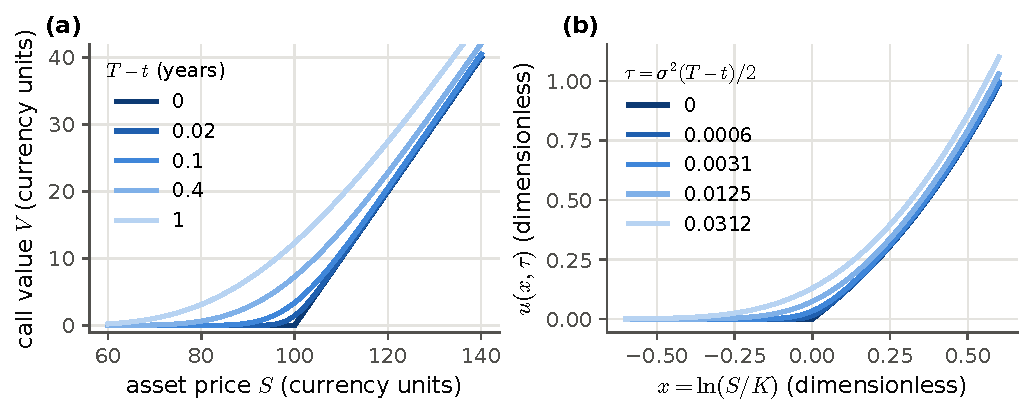
\includegraphics[width=\textwidth]{fig_smoothing.pdf}\\[2pt]
  {\small (a) call value $V$ for several times to expiry \quad (b) the same functions as $u(x,\tau)$}
  \note{Left is the option price as we move away from expiry; right is the same thing in heat coordinates.
  The kinked payoff is an initial temperature profile, and the price today is that temperature after
  diffusion. This is the picture behind the whole project.}
\end{frame}

\begin{frame}{Uniqueness}
  \begin{theorem}[Weak maximum principle]
    If $u_\tau-u_{xx}\le0$ in $U_T=(a,b)\times(0,T_0]$ and $u$ is continuous on $\overline{U_T}$, then
    $\max_{\overline{U_T}}u=\max_{\Gamma_T}u$ ($\Gamma_T$: bottom and sides).
  \end{theorem}
  \textbf{Proof.} Let $w=u+\varepsilon x^2$, so $w_\tau-w_{xx}\le-2\varepsilon<0$. At an interior
  (or top) maximum $w_\tau\ge0$ and $w_{xx}\le0$, so $w_\tau-w_{xx}\ge0$: a contradiction. Hence
  $\max u\le\max_{\Gamma_T}u+\varepsilon\max(a^2,b^2)$; let $\varepsilon\to0$. \hfill$\square$
  \vspace{4pt}
  \begin{itemize}
    \item \textbf{Bounded interval:} the difference $w$ of two solutions is $0$ on $\Gamma_T$; apply the
      theorem to $\pm w$ $\Rightarrow$ $w\equiv0$.
    \item \textbf{Whole line:} unique if $|u|\le Ae^{ax^2}$; Tychonoff's example shows that some growth
      condition is necessary. Our $u$ grows only like $e^{c|x|}$.
  \end{itemize}
  \note{The maximum principle says heat cannot create a new hottest point inside the domain. Applied to the
  difference of two solutions it gives uniqueness on an interval. On the whole line we need a growth
  condition, and our solution satisfies it, so the Black--Scholes price is unique.}
\end{frame}

\begin{frame}{Solving for the call: complete the square}
  $u_0=0$ for $s<0$, so $u=I_+-I_-$ with
  \[
    I_\pm=\frac{1}{\sqrt{4\pi\tau}}\int_0^\infty e^{\frac{k\pm1}{2}s}e^{-(x-s)^2/4\tau}\dd s .
  \]
  Substitute $s=x+\sqrt{2\tau}\,y$ (so $\frac{(x-s)^2}{4\tau}=\frac{y^2}{2}$), $m_\pm=\frac{k\pm1}{2}\sqrt{2\tau}$:
  {\small
  \[
    I_\pm=\frac{e^{\frac{k\pm1}{2}x}}{\sqrt{2\pi}}\int_{-x/\sqrt{2\tau}}^\infty e^{-\frac12y^2+m_\pm y}\dd y,\qquad
    -\tfrac12y^2+m_\pm y=-\tfrac12(y-m_\pm)^2+\tfrac12m_\pm^2 .
  \]}
  \begin{block}{Result}
    \[
      I_\pm=e^{\frac{k\pm1}{2}x+\frac{(k\pm1)^2}{4}\tau}\,\N(d_\pm),\qquad
      d_\pm=\frac{x}{\sqrt{2\tau}}+\frac{k\pm1}{2}\sqrt{2\tau}
    \]
  \end{block}
  \note{The payoff is a difference of two exponentials, so the convolution splits into two Gaussian
  integrals. Completing the square shifts each Gaussian, and the integral becomes the normal distribution
  function N evaluated at d plus or d minus.}
\end{frame}

\begin{frame}{Back to prices: the Black--Scholes formula}
  Undo the substitution, $V=Ke^{\alpha x+\beta\tau}(I_+-I_-)$:
  \begin{itemize}
    \item $I_+$: $\alpha+\frac{k+1}{2}=1$, $\beta+\frac{(k+1)^2}{4}=0$ $\Rightarrow$ prefactor $Ke^x=S$.
    \item $I_-$: $\alpha+\frac{k-1}{2}=0$, $\beta+\frac{(k-1)^2}{4}=-k$ $\Rightarrow$ prefactor
      $Ke^{-k\tau}=Ke^{-r(T-t)}$.
    \item $\sqrt{2\tau}=\sigma\sqrt{T-t}$ turns $d_\pm$ into $d_{1,2}$.
  \end{itemize}
  \begin{block}{Theorem (Black--Scholes, 1973)}
    \[
      V(S,t)=S\,\N(d_1)-Ke^{-r(T-t)}\N(d_2),\qquad
      d_{1,2}=\frac{\ln\frac SK+(r\pm\frac{\sigma^2}{2})(T-t)}{\sigma\sqrt{T-t}}
    \]
  \end{block}
  {\small Checks: put--call parity (gap $\le\parityGap$); $V\to0$ as $S\to0$; $V\to\max(S-K,0)$ as $t\to T$.}
  \note{The exponents combine exactly: the first term becomes S, and the second becomes the discounted
  strike. This is the Black--Scholes formula, derived purely from the heat kernel. The limits and put--call
  parity check out to machine precision.}
\end{frame}

\begin{frame}{Numerical check}
  \centering
  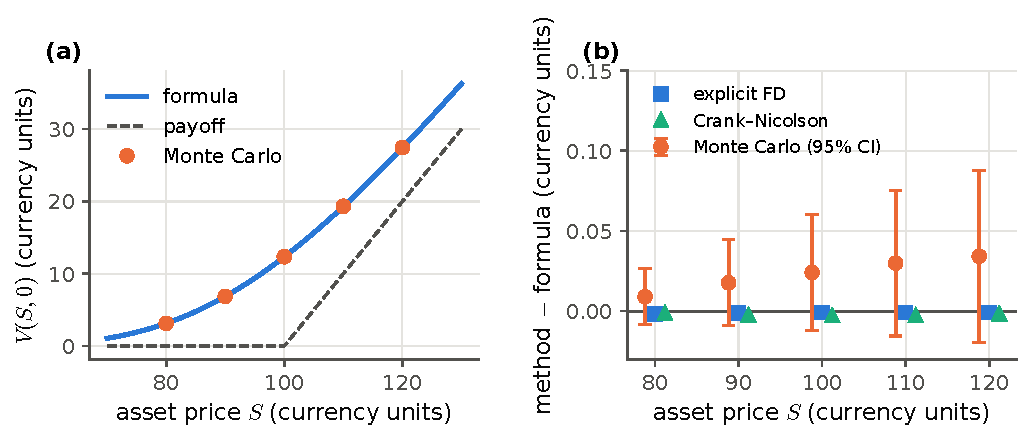
\includegraphics[width=\textwidth]{fig_methods.pdf}\\[2pt]
  {\small $V(100,0)=\priceHundred$. Heat-kernel quadrature agrees to $\errHeatKernel$, finite differences
  to $\errExplicit$; Monte Carlo ($10^6$ paths) lies inside its 95\% CI.}
  \note{We price the same option four ways. Numerical quadrature of the heat kernel reproduces the formula to
  rounding error, the finite-difference schemes to a few thousandths, and Monte Carlo lies within its
  confidence interval at every price.}
\end{frame}

% =====================================================================
\section{Applications: barriers, numerics, machine learning}

\begin{frame}{Double-barrier option: separation of variables}
  Knocked out if $S$ hits $B_1=\Bone$ or $B_2=\Btwo$: \ $u(a,\tau)=u(b,\tau)=0$, with
  $a=\ln\frac{B_1}{K}$, $b=\ln\frac{B_2}{K}$, $\ell=b-a$.
  \vspace{4pt}

  $u=X(x)\Theta(\tau)$ $\Rightarrow$ $\dfrac{\Theta'}{\Theta}=\dfrac{X''}{X}=-\lambda$:
  \[
    X''+\lambda X=0,\quad X(a)=X(b)=0 .
  \]
  \begin{itemize}
    \item $\lambda\le0$: only $X\equiv0$.\quad $\lambda>0$: $\sin(\sqrt\lambda\,\ell)=0$ $\Rightarrow$
      $\lambda_n=(n\pi/\ell)^2$.
  \end{itemize}
  \begin{block}{Fourier sine series}
    \[
      u=\sum_{n\ge1}c_n\sin\frac{n\pi(x-a)}{\ell}e^{-\lambda_n\tau},\qquad
      c_n=\frac2\ell\int_{\max(a,0)}^b u_0\sin\frac{n\pi(x-a)}{\ell}\dd x
    \]
  \end{block}
  \note{The barriers become zero boundary values on an interval, the classic separation-of-variables
  setting. The eigenvalue problem has only sine solutions, and the coefficients follow from orthogonality.
  The lower limit is max of a and zero because the payoff vanishes below the strike.}
\end{frame}

\begin{frame}{Double-barrier option: results}
  \centering
  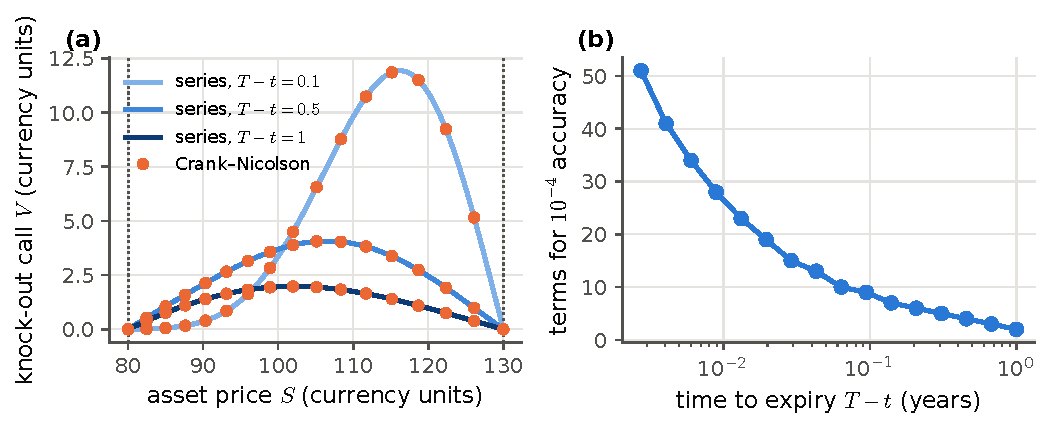
\includegraphics[width=\textwidth]{fig_barrier.pdf}\\[2pt]
  {\small The series matches Crank--Nicolson to $\barDiffMax$. Terms for $10^{-4}$ accuracy:
  \termsLongest{} at one year, \termsShortest{} at one day; $N\propto(T-t)^{-1/2}$.}
  \note{The series and an independent Crank--Nicolson solution agree to about ten to the minus five. Near
  expiry the high modes have not decayed yet, so many terms are needed; the count grows like one over the
  square root of time to expiry, as the decay factor predicts.}
\end{frame}

\begin{frame}{Explicit scheme and von Neumann stability}
  \begin{columns}[c]
    \begin{column}{0.45\textwidth}
      {\small
      \[
        u_j^{m+1}=u_j^m+\lambda\big(u_{j+1}^m-2u_j^m+u_{j-1}^m\big)
      \]}
      $\lambda=\Delta\tau/\Delta x^2$. Insert $u_j^m=G^me^{i\xi j\Delta x}$:
      \[
        G=1-4\lambda\sin^2\tfrac{\xi\Delta x}{2}
      \]
      \[
        |G|\le1\ \forall\xi\iff\lambda\le\tfrac12
      \]
    \end{column}
    \begin{column}{0.55\textwidth}
      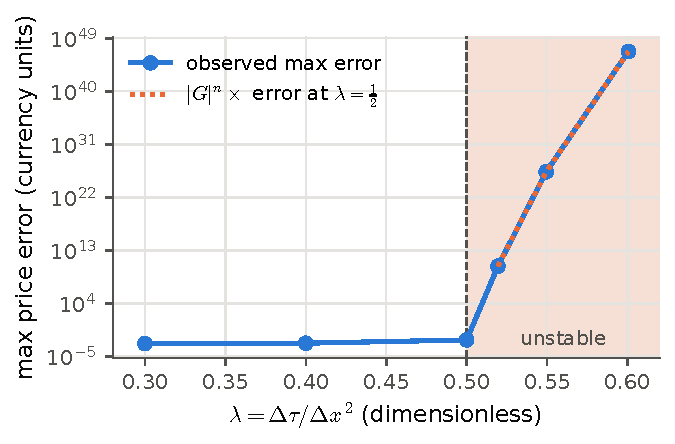
\includegraphics[width=\textwidth]{fig_stability.pdf}
    \end{column}
  \end{columns}
  \note{The worst mode is the sawtooth, with G equal to one minus four lambda, which leaves the unit
  interval exactly when lambda exceeds one half. In the experiment the error jumps from about
  \stabErrForty{} at 0.4 to \stabErrFiftyTwo{} at 0.52.}
\end{frame}

\begin{frame}{Convergence order}
  \begin{columns}[c]
    \begin{column}{0.42\textwidth}
      Truncation error:
      \[
        \Delta x^2\Big(\tfrac\lambda2-\tfrac1{12}\Big)u_{xxxx}
      \]
      Observed order at $\lambda=0.4$: \textbf{\convOrderMax}.\\[6pt]
      The payoff kink causes no loss (kink off a node: $\convOrderOff$).
    \end{column}
    \begin{column}{0.58\textwidth}
      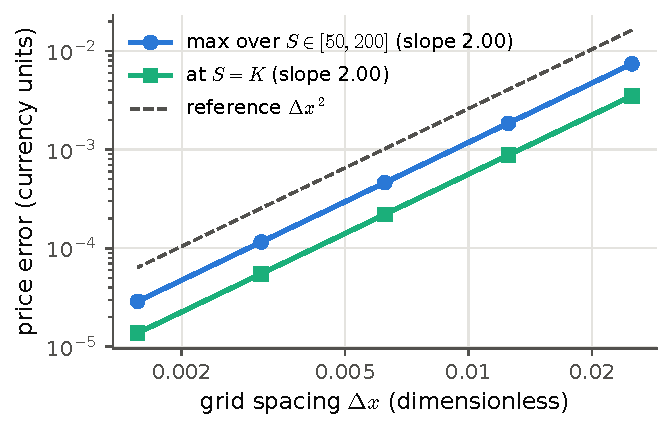
\includegraphics[width=\textwidth]{fig_convergence.pdf}
    \end{column}
  \end{columns}
  \note{Halving dx divides the error by four, so the scheme is second order. The kink did not degrade it,
  because a kink's Fourier transform decays like one over xi squared and the scheme damps the high
  modes.}
\end{frame}

\begin{frame}{Machine learning: plain network vs PINN}
  \centering
  {\small Inputs $(S/K,\,T-t)$, output $V/K$; MLP, \nnDepth{} hidden layers of \nnWidth{} $\tanh$ units.\\
  PINN loss $=$ data $+\ \|\text{PDE residual}\|^2$ $+$ terminal $+$ boundary}\\[4pt]
  {\small\begin{tabular}{ccccc}
    \toprule
    & \multicolumn{2}{c}{price RMSE} & \multicolumn{2}{c}{mean $|$residual$|$}\\
    \cmidrule(lr){2-3}\cmidrule(lr){4-5}
    $N$ & plain & PINN & plain & PINN\\
    \midrule
    \TableNNRowsShort
    \bottomrule
  \end{tabular}}\\[4pt]
  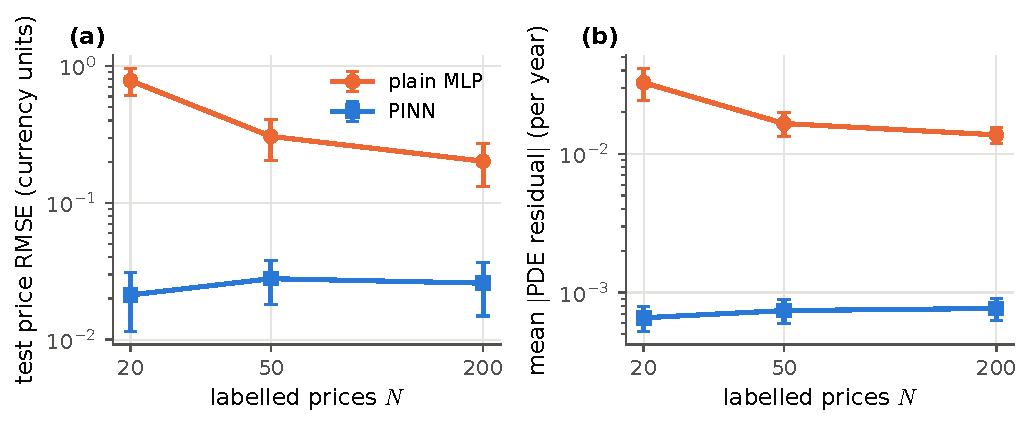
\includegraphics[height=0.33\textheight]{fig_nn.pdf}
  \note{The plain network fits its few labels but violates the PDE in between. The PINN also penalises the
  PDE residual, computed by automatic differentiation, and with 20 labels it is about
  \nnRmseRatioTwenty{} times more accurate.}
\end{frame}

\begin{frame}{Limitations and ill-posedness}
  \begin{itemize}
    \item Constant $\sigma$ and $r$; no jumps, no dividends.
    \item Must be solved backwards: forward in $t$ it is the backward heat equation.
  \end{itemize}
  \centering
  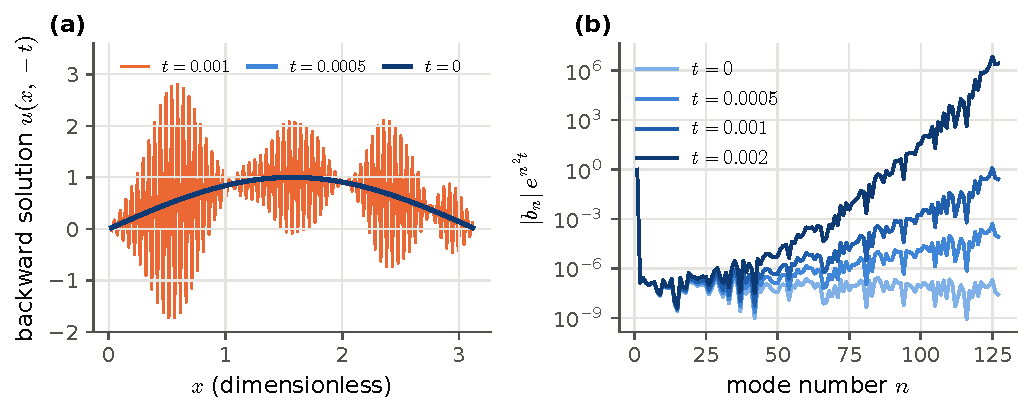
\includegraphics[width=0.95\textwidth]{fig_illposed.pdf}\\[2pt]
  {\small Noise of size $\illEps$ grows to $\illMaxNoisyTwoMilli$ after backward time $0.002$.}
  \note{The reduction needs constant volatility and rate; jumps give an integro-differential equation.
  Running the heat equation backwards multiplies mode n by e to the n squared t, so noise of size one in a
  million explodes within a few thousandths of a time unit.}
\end{frame}

\begin{frame}{Conclusions}
  \begin{enumerate}
    \item Black--Scholes is parabolic, degenerate at $S=0$, and a terminal-value problem.
    \item Three substitutions turn it into $u_\tau=u_{xx}$.
    \item The heat kernel gives the Black--Scholes formula.
    \item Barrier options give a Fourier sine series.
    \item Explicit finite differences: stable iff $\lambda\le\frac12$, order 2.
    \item Adding the PDE to the loss beats adding more data.
  \end{enumerate}
  \note{Every result follows from the heat equation: smoothing, the formula, the barrier series, the
  stability limit and the danger of solving in the wrong direction. The neural network experiment shows the
  PDE is useful even when we only want to fit data.}
\end{frame}

\begin{frame}{References}
  \footnotesize
  \begin{itemize}
    \item L.~C.~Evans, \emph{Partial Differential Equations}, AMS.
    \item T.~Myint-U, L.~Debnath, \emph{Linear PDEs for Scientists and Engineers}, Birkhäuser.
    \item R.~C.~McOwen, \emph{Partial Differential Equations: Methods and Applications}.
    \item A.~K.~Nandakumaran, P.~S.~Datti, \emph{Partial Differential Equations}, CUP.
    \item F.~Black, M.~Scholes, J.\ Political Economy 81 (1973).
    \item P.~Wilmott, S.~Howison, J.~Dewynne, \emph{The Mathematics of Financial Derivatives}, CUP (1995).
    \item M.~Raissi, P.~Perdikaris, G.~E.~Karniadakis, J.\ Comput.\ Phys.\ 378 (2019).
  \end{itemize}
  \vfill
  \centering\Large Thank you! Questions?
\end{frame}

\end{document}
